Implementacija vezji je proces pretvarjanja načrta za vezje v dejansko vezje, ki obdeluje vhodne podatke in oddaja izhodne podatke. Obstajajo različni načini implementacije digitalnih vezji

\begin{itemize}
	\item Simulacija
	\item FPGA
	\item Integrirana vezja
\end{itemize}

\subsection{Simulacija}
Simulacija je najpreprostejši način implementacije. Slaba stran simulacije je, da niso upoštevane časovne lastnosti realnih implementacij, kar je v primeru asinhronih vezji zelo pomembne.
Slabost je tudi dejstvo, da simulirano vezje ni uporabno za samo obdelavo podatkov.

\subsection{Integrirana vezja}
Integrirana vezja so končna faza implementacije elektronskih vezji. Pri izdelavi integriranih vezji imamo največ nadzora, zato lahko zagotovimo nekaterim časovnim predpostavkam, ki jim sicer ne moramo. Slaba stran je visoka cena izdelava.

\subsection{FPGA}
Implementacija v FPGA je privlačna, saj nima visoke cene in hkrati dobimo dejansko vezje na katerem lahko pomerimo časovne in ostale karakteristike.
Slabosti FPGA implementacije pa je, da nimamo preciznega nadzora nad časovnimi karakteristikami in primitivi, ki so nam na voljo.


Za to magistersko nalogo smo se odločili za implementacijo v vezju FPGA, saj predstavlja srečno srednjo pot.

\section{Arhitektura FPGA} \label{a}
FPGA so vezja za implementacijo specializirane logike.

Sestavljena so iz množice logičnih celic, ki jih povezuje matrika programibilnih povezav.


\subsection{Logične celice}
Logične celice so kosi ligitalne logike v FPGA vezjih, ki opravljajo funkcijo obdelave podatkov. Pogosto so narejene iz kombinatoričnega in spominskega dela. Kombinatorični del je zadolžen za samo obdelvo podatkov, spominski del pa za urejen pretok samih podatkov.

\begin{figure}
	\centering
	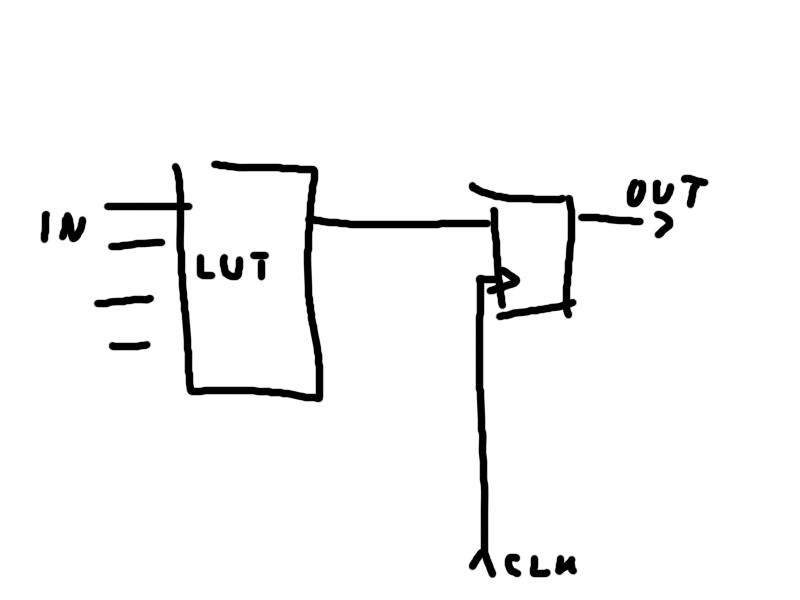
\includegraphics[width=0.7\linewidth]{slike/cell}
	\caption{}
	\label{fig:cell}
\end{figure}

\subsubsection{Kombinatorični del}
Kombinatorični del je implementiran kot iskalne tabele. To so kosi spomina, ki so sprogramirani ob zagonu vezja. V njih je sprogramirana pravilnostna tabela kombinatoričnega vezja.

\subsubsection{Spominski del}
Spominski del je implementiran kot konfigurabilna flip-flop celica, kateri lahko nastavimo polariteto, ali je zapah ali register ima reset in preset itd.


\subsection{Povezave}
Povezave zagotovijo možnost da se katera koli celica poveže z katero koli drugo celico v FPGA vezju. Matrika povezav je narejena iz mreže programibilnih križišč, ki so povezana s svojimi sosedi. Te lahko povežejo arbitrarna križišča med seboj. Na vsako križišče je povezana tudi logična celica. Taka arhitektura nam dovoli izjemno fleksibilnost a ne pride brez slabosti. Ker so povezave programibilne, pomeni, da imajo relativno veliko kapacitivnost, kar upočasni hitrost vezja.


\begin{figure}
	\centering
	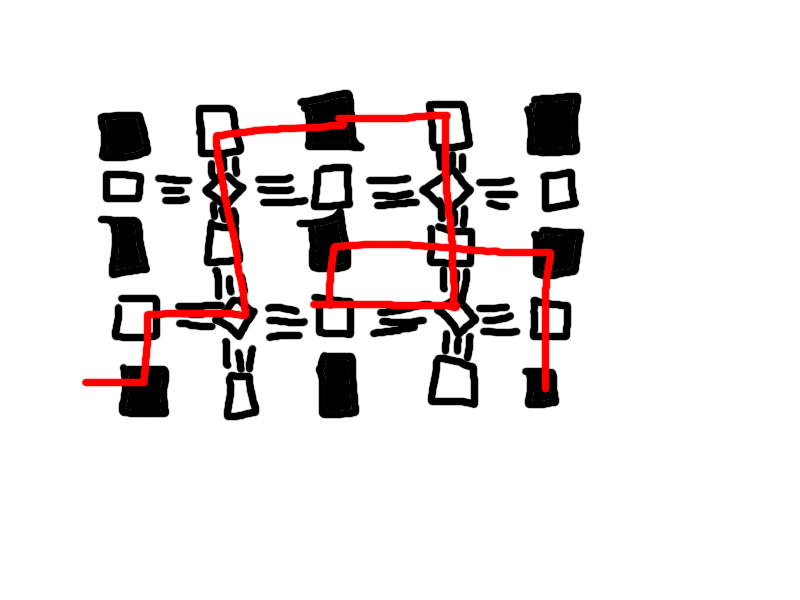
\includegraphics[width=0.7\linewidth]{slike/routing}
	\caption{}
	\label{fig:cell}
\end{figure}


\subsection{Vgrajeni bloki}
Pogosto imajo FPGA vezja tudi dodatne funkcionalnosti, ki pohitrijo pogoste primere uporabe.

\begin{itemize}
	\item \textbf{Prenosne verige}: hitre povezave med logičnimi bloki, uporabljene za ustvarjanje logike z velikim številom vhodov npr. seštevalniki
	\item \textbf{Globalne linije}: Povezave za uro in reset so ponavadi globalne, zato imajo nekatrea FPGA vezja posebne povezave za take signale. Urni signal potrebuje posebno pozornost, saj mora vse celice zadeti z čim manjšo razliko v zakasnitvah.
	\item \textbf{Specializirani bloki}: Pogosti gradniki digitalih vezji, ki zasedejo veliko prostora kot npr. množilniki in spominski bloki so ponavadi vgrajeni direktno v FPGA, da prihranimo logične celice. Nekatra FPGA vezja imajo tudi celotna procesorska jedra direktno vgrajena.
\end{itemize}



\subsection{Vhodi in izhodi}

Pomemben del FPGA vezji so tudi izhodi in vhodi. Ti so povezani na posebne bloke ki ojačajo signale, tako da so primerni za zunanje okolje. ZAgotovijo tudi sposobnost stanja visoke impedance. Pomembno je tudi, da se signali ob vstopu v vezje sinhronizirajo na notranju urni takt. Večina izhodov in vhodov so navadne digitalne povezave. Nekatera FPGA vezja imajo tudi posebne izhode in vhode za posebne protokole kot npr. PCI-E, DDR itd.



\section{Implementacija} \label{a}
Za implentacijo vezji v FPGA je potrebno spisati opis vezja v enem izmed jezikov za opis vezji(HDL). To je ponavadi (system)verilog ali VHDL. Nato programsko orodje prevede ta opis vezja v konkreten načrt tega vezja v FPGA vezju.

Cilj tega magisterskega dela je izdelava asinhronih vezji v FPGA vezjih. Problem je, da so FPGA vezja namenjena izdelavi sinhronih vezji. Velikokrat povezave med logičnimi elementi niso narejene kakor bi pričakovali, ne moramo se zanašati na zakasnitve v vezju. Večina implementacij asinhronih vezji v FPGA zato eksplicitno določi postavitev logičnih elementov in njihovih povezav v vezju. Taksen pristop deluje za manjša vezja vendar, ko vezja postanejo večja postane zelo časovno potraten. 

Namesto da ročno diktiramo povezave, da zagotovimo predpostavkam, raje uporabimo asinhroni stil, kjer so predpostavke dovolj šibke, da se lahko zanesemo, da bodo izpolnjene brez dodatnih navodil.
Zato se odločimo za dual-rail asinhroni stil. 


\subsection{SystemVerilog} \label{b}
Odločili smo se za implementacijo v jeziku SystemVerilog. Systemverilog je jezik, ki se uporablja za zasnovo in simulacijo digitalnih elektronskih vezji. Uporablja se za zasnovo vezji, ki so implementirana v FPGA.


\subsection{Knjižnica} \label{b}
Izdelali smo knjižnico v jeziku systemverilog, za izdelavo asinhronih vezji v FPGA. Knjižnica je sestavljena hierarhično

\begin{enumerate}
	\item Osnovni gradniki
	\item Funkcionalne enote
	\item Vezja
\end{enumerate}

Implementirali smo knjižnico za 4 fazen in 2 fazen stil. Kljub tem, da imajo elementi indentične vhode in izhode moramo biti pazljivi, saj štirifazna vezja ne podpirajo ciklov krajših od 3 elementov medtem, ko so lahko v dvofaznih vezjih tudi obroči z dvema elementoma.


\subsection{4-Phase dual rail} \label{b}
Štirifazna vezja implementiramo z NCL logiko. Za zapahe uporabimo mousetrap registre, ker so lepše implementirani v FPGA vezjih.

NCL logika uporablja nivojsko logiko, za izdelavo kombinatoričnih vezji. Za pravilno ponastavitev poskrbi histerezni karakter, ki poskrbi da se ničelna vrednost pravilno propagira skozi vezje.

\subsubsection{Nivojska logika} \label{c}
TODO



\subsection{2-Phase dual rail} \label{b}
Dvofazna vezja tudi uporabljajo mousetrap zapahe, vendar za kombinatorična vezja uporablja metodo bližjo naivni logični sintezi

Princip je, da zaznamo vse možne kombinacije vhodnih preklopov. Nato resetiramo te vhode in pošlenmo izhode TODO bolj natančno



\subsection{Workcraft} \label{b}
Workraft je programsko orodje za delo z grafnimi modeli. Uporabno je za zasnovo in sintezo gradnikov asinhronih vezji, kot tudi za simulacijo arhitekture raznih asinhronih vezji.

\subsubsection{Sinteza gradnikov} \label{b}
Željeno vezje opišemo z uporabo grafa signalnih preklopov(STG). V tem grafu določimo zaporedje preklopov vhodnih in izhodnih signalov, ki določajo delovanje vezja. Za C element na primer, določimo da preklopu obeh vhodov sledi preklop izhoda. Iz tega grafa orodje sestavi vezje, ki se obnaša tako kot graf, ki ga opisuje.

\subsubsection{Simulacija arhitekture asinhronih vezji} \label{b}
Za simulacijo vezji uporabimo graf signalnih preklopov(STG) oz. graf podatkovnega poteka(DFS) odvisno od stila implementacije. Za dvofazna vezja, je bolj primeren STG, saj modelira preklope, medtem ko je za štirifazna vezja bolj primeren DFS, saj upošteva ponastavitvani val, ki sledi podatkovnem valu. Te simulacije so uporabne, saj z njimi lahko preverimo, da se podatki po vezju pretakajo kot smo si to zamislisi.




\subsection{Implementacija cellic} \label{a}
Knjižnica implementira vse potrebne primitive za izdelavo poljubnih asinhronih vezji.


\subsubsection{Primitivi} \label{b}
Imamo 2 Primitiva. Primitivi so implementirani direktno z FPGA primitivi, da zagotovimo, da delujejo pravilno.

\begin{itemize}
	\item Muller C element. Klasični element implementiran z pravilnostno tableo.TODO test portable
	\item Nivojska vrata. Implemetirana direktno z pravilnostno tabelo. TODO test portable
\end{itemize}

\subsubsection{Osnovne celice} \label{b}
Osnovne celice so implementirane direktno v SystemVerilog kodi, in so prenosne na kateri koli FPGA. So najnižja stopnja v hierarhiji, zato lahko vsebujejo le druge osnovne celice.

\begin{itemize}
	\item TOGGLE. Element za dvofazna vezja. Sintetiziran s pomočjo programa workcraft. 
\end{itemize}


\subsubsection{Funkcionalne celice} \label{b}
Funkcionalne celice so sestavljene iz osnovnih celic in dodatne povezovalne logike. To so celice, ki imajo neko konkretno funkcijo kot npr. zapahi, splošni C elementi itd. 


\begin{itemize}
	\item Registri. 
\end{itemize}


\subsubsection{Logika} \label{b}
To so končani kombinatorični sklopi, ki jih lahko vmestimo direktno med registre

\begin{itemize}
	\item AND,OR. 
	\item FULL ADDER. 
	\item ect. 
\end{itemize}

\subsubsection{Vezja} \label{b}
Končana vezja, ki opravljajo določeno nalogo. Te se razlikujejo med dvofanimi in štirifaznimi implementacijamo

\begin{itemize}
	\item PIPELINE. 
	\item COUNTER. 
	\item FIBBONACCI. 
	\item GCD. 
\end{itemize}





